\documentclass{article}
\usepackage{hyperref}
\usepackage{amsmath,amssymb}
\usepackage{graphicx}
\usepackage{caption}
\usepackage{subcaption}
\usepackage{color}
\usepackage[section]{placeins}
\usepackage{listings}


\title{Combustion Theory Final Take Home Exam} 
\author{Nicholas Malaya\\ Department of Mechanical Engineering \\
University of Texas at Austin}  
\date{}

\begin{document}
\maketitle
\newpage


\section*{Turbulent diffusion flames}

In this problem, I want you to assume that the system is turbulent and
that you know the turbulence mass diffusivity ($D_T$) is 10 times the
laminar value. Assume that the fluctuation squared of the mixture
fraction is equal to the gradient of the mean mixture fraction squared
multiplied by the characteristic diffusion length scale squared, i.e.
\begin{equation}
 \bar{z'z'} = \frac{1}{2} (\nabla \bar z)^2 \frac{D_T L_x}{u}
\end{equation}

\subsection*{a) Write down the solution for the mean mixture fraction field
  with the turbulent diffusivity.}

We start with the steady state species equation, 
\begin{equation}
 \rho u \frac{\partial Y_i}{\partial x} = \rho D \frac{\partial^2
  Y_i}{\partial y^2} \pm \omega_i. 
\end{equation}
We note that, 
\begin{equation}
 \omega = \frac{\omega_i}{\nu_i W_i} = \frac{\omega_F}{\nu_F W_F} =
  \frac{\omega_O}{\nu_O W_O}. 
\end{equation}
This hints at a conserved scalar form of the species equation, where
with, 
\begin{equation}
 \beta  = \frac{\omega_F}{\nu_F W_F} - \frac{\omega_O}{\nu_O W_O}
\end{equation}
then our reaction is decoupled from the convection-diffusion of a
conserved scalar quantity. In particular, 
\begin{equation}
 \mathcal{L}(\beta)  = \mathcal{L}\left(\frac{\omega_F}{\nu_F W_F} -
				   \frac{\omega_O}{\nu_O W_O} \right)
 \Rightarrow \rho u \frac{\partial \beta_i}{\partial x} - \rho D \frac{\partial^2
  \beta_i}{\partial y^2} = 0. 
\end{equation}
Now, we construct z, 
\begin{equation}
 z = \frac{\beta -\beta_{O}}{\beta_F - \beta_{O}}
\end{equation}
Here, the boundary conditions are that $z=1$ for all $y>0$ and $x<0$
(e.g. the fuel reserve) and $z=0$ for $y<0$ and $x<0$ (e.g. the oxygen
reserve). 

Thus, we are solving, 
\begin{equation}
\rho u \frac{\partial z}{\partial x} - \rho D \frac{\partial^2
  z}{\partial y^2} = 0. 
\end{equation}
and, 
\begin{equation}
\rho u \frac{\partial \bar z}{\partial x} - \rho D_T \frac{\partial^2
  \bar z}{\partial y^2} = 0. 
\end{equation}
Where the first equation is from the laminar flow, and the latter case
is the favre-averaged mean field. We now need to discretize this equation, 
in order to solve it numerically (It looks like it would be a trainwreck to solve
analytically!). We will completely wimp out, and only use finite difference methods, 
\begin{align}
  \frac{\partial \bar z}{\partial x} &= \frac{\bar z_{i+1}-\bar z_{i}}{\Delta x} \\
  \label{first}
  \frac{\partial^2 \bar z}{\partial y^2} &= \frac{\bar z_{j+1}-2\bar z_{j}+\bar z_{j-1}}{\Delta y^2} 
\end{align}
The boundary conditions are $\bar z = 1$ $\forall x<0,y>0$, $\bar z = 0$ $\forall x<0,y<0$. 
I additionally imposed a Neuman (zero flux) boundary condition on the top and bottom of the box, 
essentially forcing the derivatives to zero at $\pm \infty$. As with the previous examination, 
we are now in a position to instantiate this on a computer using python to solve for 
the $\bar z(x,y)$ field. 

As an interesting implementation detail, because the solution is only
first order in x, we only need one boundary condition for that
direction, as shown above. This is equivalent to an initial condition on
a first order (in time) ODE. Thus, we do not actually need to store our
entire x-domain in memory, but can simply solve for all y-values at our
particular x-coordinate, and then step forward in space and solve for
the next grid location. 

%
%
%
%
\subsection*{b) Plot the fluctuation and mean value of the mixture fraction
  at 5 cm, 30 cm, and 50 cm.}

  \begin{figure}[!htb]
   \begin{center}
    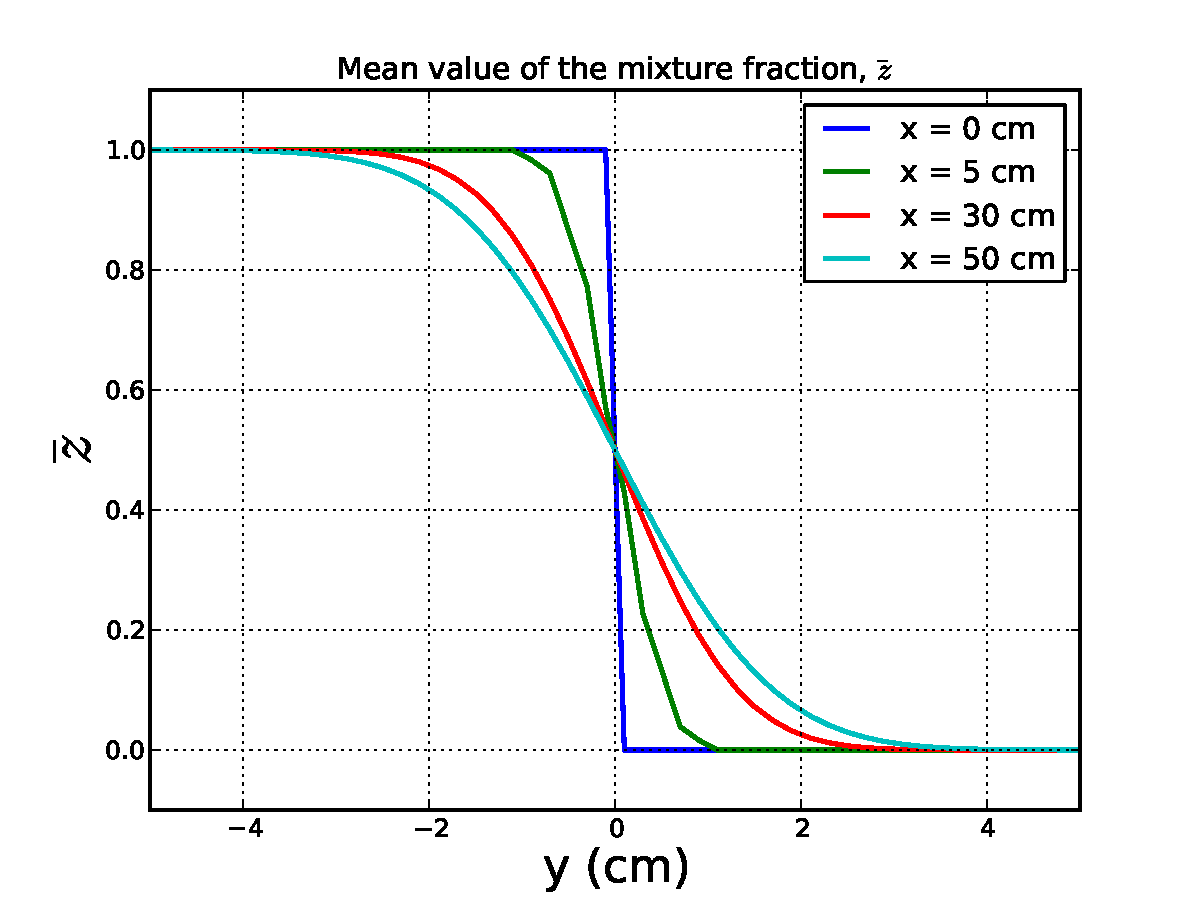
\includegraphics[width = 12 cm]{figs/mean.pdf}
    \caption{The mixture fraction plotted as a function of y.}
    \label{mean}
   \end{center}
   \end{figure}

The method to arrive at the mean value mixture fraction was described
above. The value of the mixture fraction at several locations is plotted
in figure \ref{mean}. The flow at $x=0$ cm is a sharp interface between
the fuel and the oxidizer. As you move downstream, the fuel and oxidants 
mix, which will create a mixing layer that diffuses out and increases in
y-width as a function of distance downstream. 

The fluctuation $\bar{z'z'}$
must also be determined. Normally, this would require solving another differential equation, 
and potentially using submodels for the scalar dissipation rate as well. However, we were given a
simplified expression (model) for the variance, namely,
\begin{equation}
 \bar{z'z'} = \frac{1}{2} (\nabla \bar z)^2 \frac{D_T L_x}{u}. 
\end{equation}
Variations in y will be much larger than variations in x, and this expression 
can be simplified to be,
\begin{equation}
 \bar{z'z'} = \frac{1}{2} (\frac{\partial \bar z}{\partial y})^2 \frac{D_T L_x}{u}. 
 \label{fluc}
\end{equation}
This expression is a model for the variance of the mixture
fraction. Intuitively, this expression is reasonable,  as we expect the
variance (in some sense, our uncertainty) of the value of the mixture
fraction to be largest in regions with large gradients. In the mixing
layer, the gradient will be quite large near the layer ($y=0,x=0$) and expanding outward  at larger x. 

We discretize equation \ref{fluc} using the finite difference scheme
shown in equation \ref{first}, however, now the indicies are changed
from i to j, to reflect the different direction of the
derivative. However, upon running the code, I found that a forward
finite difference was very numerically noisy for the solution at $x=5$
cm. This was because the interface at this distance is still quite
sharp, and so squaring the derivative ``blew-up'' the noise. I therefore
switched a centered finite difference scheme, namely:
\begin{equation}
  \frac{\partial \bar z}{\partial y} = \frac{\bar z_{i+1}-\bar z_{i-1}}{2\Delta y}.
\end{equation}

  \begin{figure}[!htb]
   \begin{center}
    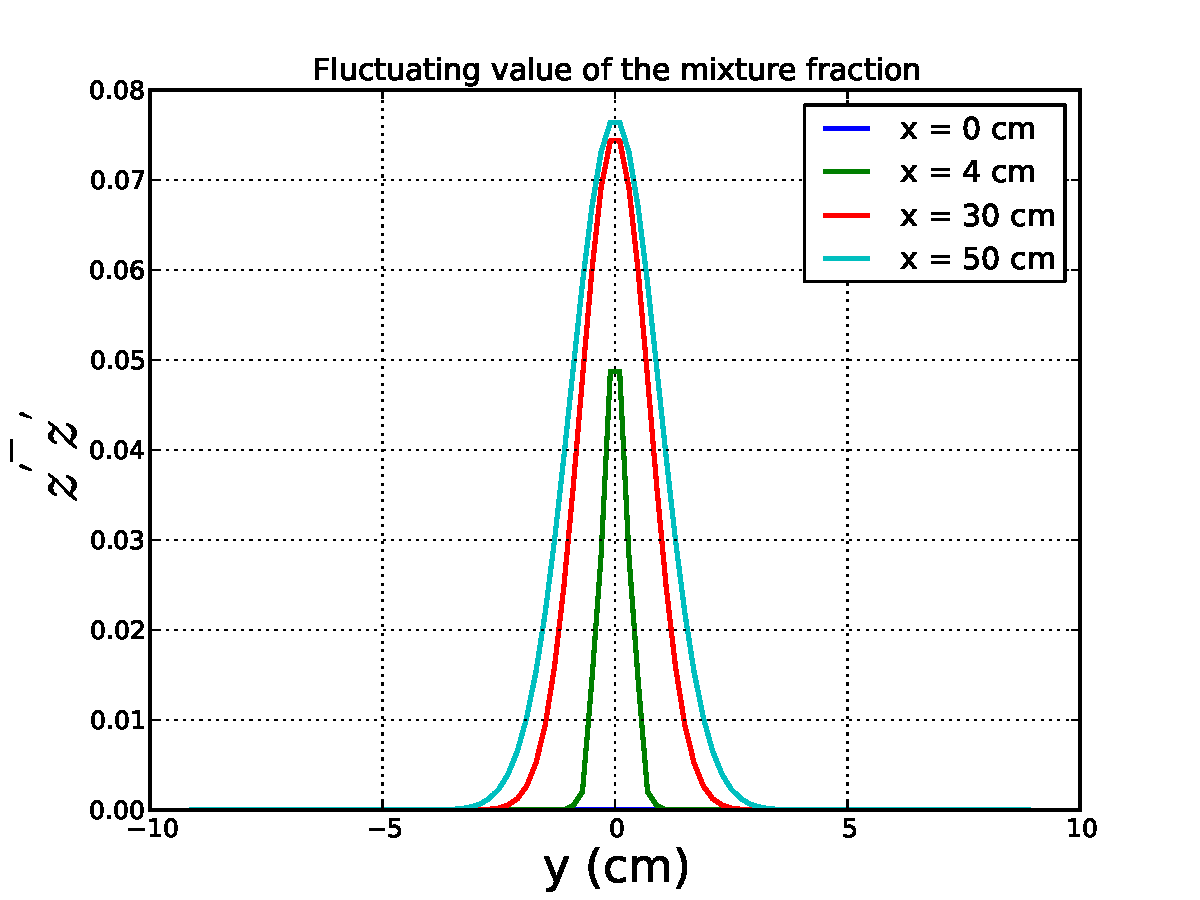
\includegraphics[width = 12 cm]{figs/fluc.pdf}
    \caption{The mixture fraction variance plotted as a function of y.}
    \label{fluc}
   \end{center}
  \end{figure}

The results are plotted in figure \ref{fluc}. The results of this figure
display that at anything but low values of x, the variance is nearly
zero. It is only near the sharp interface that the flow is
turbulent. Outside of just a few centimeters, the variance is very
nearly zero, implying essentialy laminar flow. As we move downstream,
the pdf opens up, as the mixing layer grows and entrains more fluid
around it. The peak also grows, implying that the turbulence grows to a
higher reynolds number, with larger fluctuations. 

%
%
%
%
\subsection*{c) Plot the PDF of the mixture fraction at two points, $y=0$ cm,
$x=30$ and at $y=15$ cm, $x=30$ cm.}

$P(z) =$ probability of z in $z+\Delta z$. If we knew the joint probability density function
we could calculate it directly. However, we don't know P() (the PDF). Instead, we will use 
what Peters calls the ``Presumed Shape PDF Approach''. We must pick a probability distribution. 
We are limited to two parameter distributions for the model to be closed, because we only possess 
$\bar z$ and $\bar{z'z'}$. Essentially, our choice is between a clipped Gaussian and the Beta 
function distribution. We will use the Beta distribution, as it should have much more appropriate 
limit behaviour for the mixing layer. In particular, due to the effect of intermittency, we expect the 
edges of the mixing layer to act like a delta function. This effect can be captured by the Beta distribution. 
The distribution function pdf has the form, 
\begin{equation}
P(\bar z) = \frac{\bar z^{\alpha-1}(1-\bar z)^{\beta-1}}{\Gamma(\alpha)\Gamma(\beta)}\Gamma(\alpha + \beta)
\end{equation}
We further define,
\begin{align}
\alpha &= \bar z \gamma \\
\beta  &= (1-\bar z) \gamma
\end{align}
Where the variable $\gamma$ is defined as, 
\begin{equation}
  \gamma = \frac{\bar z (1-\bar z)}{\bar{z'z'}^2} -1 \geq 0.
\end{equation}
%
%
%
%
\subsection*{d) Plot the laminar and mean turbulent temperature
distributions at $x=30$ cm.}

\subsection*{e) Discuss the results.}

A few initial comments. The entire formulation utilized chemical equilibrium models 
to find the long time stable solution. The model cannot predict extinction or ignition. 
This also assumes that the chemical time scales are much smaller than the turbulence 
time scales, e.g. that the Damkohler number is large. 

Finally, we either ``turned-on'' or ``turned-off'' the turbulence
(e.g. it was fully developed turbulence, or completely laminar). In
reality, the flow might be intermittent or laminar away from the mixing
layer at $y=0$ and turbulent near it. So a mixing of the models might be
more appropriate. Ideally, the flow would be fully turbulent near the
centerline, intermittent at the edges of the layer, and laminar outside.  

Given these assumptions, we would have to be careful using the results of 
this model in a predictive context. Those caveats aside, 

\newpage
All the work contained in this report was entirely my own. 

Thank you for the class! 
\vspace{1in}
\newline
References:

``Turbulent Combustion'', Norbert Peters

``Combustion Physics'', Chung K. Law


\end{document}
